\documentclass[tikz,border=15pt]{standalone}
\usepackage{tikz}
\usepackage{xcolor}
\usetikzlibrary{calc}

\definecolor{skyblack}{RGB}{2,6,23}
\definecolor{skynavy}{RGB}{15,23,42}
\definecolor{waterblue}{RGB}{30,27,75}
\definecolor{waterline}{RGB}{67,56,202}
\definecolor{groundblack}{RGB}{7,10,18}
\definecolor{goldlight}{RGB}{254,240,138}
\definecolor{goldspark}{RGB}{250,204,21}
\definecolor{rubyspark}{RGB}{244,63,94}
\definecolor{cyanlight}{RGB}{186,230,253}
\definecolor{cyanspark}{RGB}{56,189,248}
\definecolor{magentaspark}{RGB}{236,72,153}
\definecolor{limespark}{RGB}{163,230,53}
\definecolor{limelight}{RGB}{217,249,157}
\definecolor{purplespark}{RGB}{192,132,252}
\definecolor{lanternred}{RGB}{239,68,68}
\definecolor{lanternyellow}{RGB}{250,204,21}
\definecolor{stallred}{RGB}{220,38,38}
\definecolor{stallblue}{RGB}{2,132,199}
\definecolor{stallgreen}{RGB}{22,163,74}
\definecolor{stallbase}{RGB}{30,27,75}
\definecolor{stallpole}{RGB}{120,53,15}
\definecolor{warmglow}{RGB}{249,115,22}
\definecolor{obired}{RGB}{225,29,72}
\definecolor{obiblue}{RGB}{59,130,246}

\begin{document}
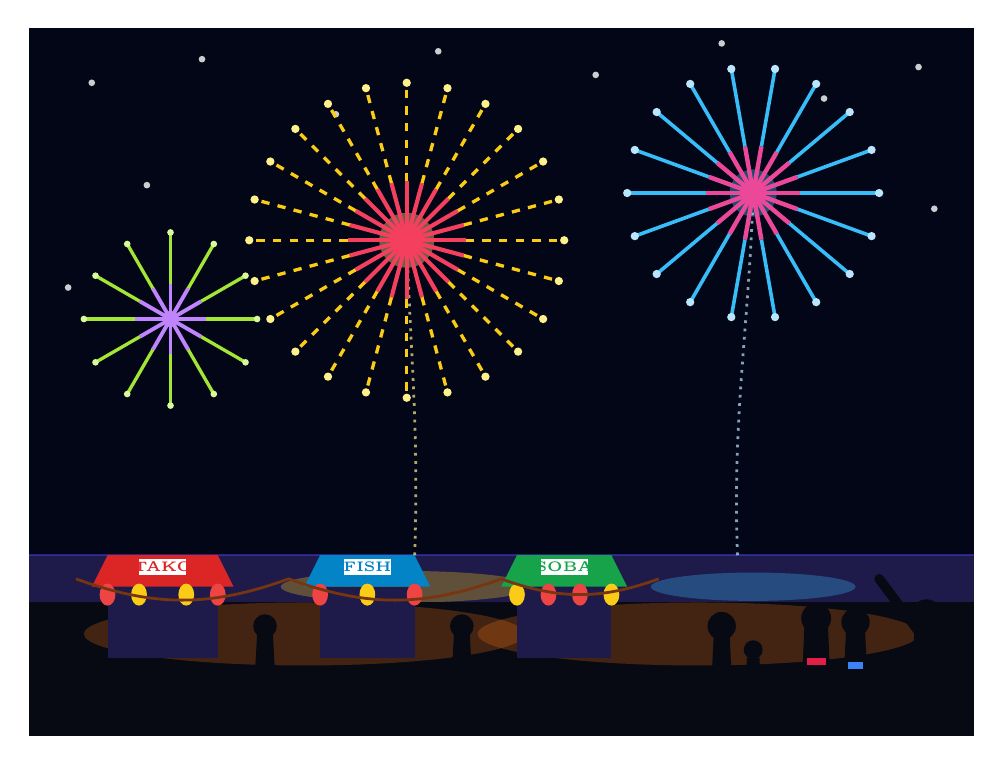
\begin{tikzpicture}

% 1. NIGHT SKY & RIVER
\fill[skyblack] (-6,-4.5) rectangle (6,4.5);
\fill[waterblue] (-6,-4.5) rectangle (6,-2.2);
\draw[waterline, line width=0.8pt, opacity=0.6] (-6,-2.2) -- (6,-2.2);

% Stars
\foreach \sx/\sy in {-5.2/3.8, -4.5/2.5, -3.8/4.1, -2.1/3.4, -0.8/4.2, 1.2/3.9, 2.8/4.3, 4.1/3.6, 5.3/4.0, 5.5/2.2, -5.5/1.2} {
    \fill[white, opacity=0.8] (\sx, \sy) circle (1.2pt);
}

% 2. FIREWORK 1: Gold Chrysanthemum (Center-Left: -1.2, 1.8, R=2.0)
\coordinate (F1) at (-1.2, 1.8);
\fill[white] (F1) circle (0.16cm);
\fill[goldlight, opacity=0.4] (F1) circle (0.35cm);

% Launch Trail 1
\draw[goldlight, dotted, line width=1pt, opacity=0.7] (-1.1, -2.2) to[out=88, in=-88] (F1);

% Spokes
\foreach \angle in {0, 15, ..., 345} {
    % Inner ruby ring
    \draw[rubyspark, line width=1.5pt] (F1) -- ($(F1)+(\angle:0.75)$);
    % Outer golden ring
    \draw[goldspark, dashed, line width=1.2pt] ($(F1)+(\angle:0.75)$) -- ($(F1)+(\angle:2.0)$);
    \fill[goldlight] ($(F1)+(\angle:2.0)$) circle (1.5pt);
}

% 3. FIREWORK 2: Cyan & Magenta (Right: 3.2, 2.4, R=1.6)
\coordinate (F2) at (3.2, 2.4);
\fill[white] (F2) circle (0.14cm);
\fill[cyanspark, opacity=0.4] (F2) circle (0.3cm);

% Launch Trail 2
\draw[cyanlight, dotted, line width=1pt, opacity=0.7] (3.0, -2.2) to[out=92, in=-92] (F2);

\foreach \angle in {0, 20, ..., 340} {
    % Inner magenta
    \draw[magentaspark, line width=1.6pt] (F2) -- ($(F2)+(\angle:0.6)$);
    % Outer cyan
    \draw[cyanspark, line width=1.3pt] ($(F2)+(\angle:0.6)$) -- ($(F2)+(\angle:1.6)$);
    \fill[cyanlight] ($(F2)+(\angle:1.6)$) circle (1.5pt);
}

% 4. FIREWORK 3: Lime & Purple (Far Left: -4.2, 0.8, R=1.1)
\coordinate (F3) at (-4.2, 0.8);
\fill[white] (F3) circle (0.1cm);
\foreach \angle in {0, 30, ..., 330} {
    \draw[purplespark, line width=1.4pt] (F3) -- ($(F3)+(\angle:0.45)$);
    \draw[limespark, line width=1.2pt] ($(F3)+(\angle:0.45)$) -- ($(F3)+(\angle:1.1)$);
    \fill[limelight] ($(F3)+(\angle:1.1)$) circle (1.2pt);
}

% 5. WATER REFLECTIONS
\fill[goldspark, opacity=0.3] (-1.2, -2.6) ellipse (1.6cm and 0.2cm);
\fill[cyanspark, opacity=0.3] (3.2, -2.6) ellipse (1.3cm and 0.18cm);
\fill[rubyspark, opacity=0.2] (-1.2, -3.1) ellipse (1.0cm and 0.12cm);
\fill[magentaspark, opacity=0.2] (3.2, -3.1) ellipse (0.8cm and 0.12cm);

% 6. FOREGROUND RIVER EMBANKMENT & STALLS
\fill[groundblack] (-6,-4.5) rectangle (6,-2.8);
\fill[warmglow, opacity=0.25] (-2.5, -3.2) ellipse (2.8cm and 0.4cm);
\fill[warmglow, opacity=0.25] (2.5, -3.2) ellipse (2.8cm and 0.4cm);

% Stall 1: Takoyaki (Left)
\fill[stallred] (-5.2, -2.6) -- (-3.4, -2.6) -- (-3.6, -2.2) -- (-5.0, -2.2) -- cycle;
\fill[stallbase] (-5.0, -3.5) rectangle (-3.6, -2.6);
\fill[white] (-4.6, -2.45) rectangle (-4.0, -2.25);
\node[text=stallred, font=\tiny\bfseries] at (-4.3, -2.35) {TAKO};
% Lanterns
\fill[lanternred] (-5.0, -2.7) ellipse (0.1cm and 0.14cm);
\fill[lanternyellow] (-4.6, -2.7) ellipse (0.1cm and 0.14cm);
\fill[lanternyellow] (-4.0, -2.7) ellipse (0.1cm and 0.14cm);
\fill[lanternred] (-3.6, -2.7) ellipse (0.1cm and 0.14cm);

% Stall 2: Kingyo-sukui (Center)
\fill[stallblue] (-2.5, -2.6) -- (-0.9, -2.6) -- (-1.1, -2.2) -- (-2.3, -2.2) -- cycle;
\fill[stallbase] (-2.3, -3.5) rectangle (-1.1, -2.6);
\fill[white] (-2.0, -2.45) rectangle (-1.4, -2.25);
\node[text=stallblue, font=\tiny\bfseries] at (-1.7, -2.35) {FISH};
\fill[lanternred] (-2.3, -2.7) ellipse (0.1cm and 0.14cm);
\fill[lanternyellow] (-1.7, -2.7) ellipse (0.1cm and 0.14cm);
\fill[lanternred] (-1.1, -2.7) ellipse (0.1cm and 0.14cm);

% Stall 3: Yakisoba (Right)
\fill[stallgreen] (0.0, -2.6) -- (1.6, -2.6) -- (1.4, -2.2) -- (0.2, -2.2) -- cycle;
\fill[stallbase] (0.2, -3.5) rectangle (1.4, -2.6);
\fill[white] (0.5, -2.45) rectangle (1.1, -2.25);
\node[text=stallgreen, font=\tiny\bfseries] at (0.8, -2.35) {SOBA};
\fill[lanternyellow] (0.2, -2.7) ellipse (0.1cm and 0.14cm);
\fill[lanternred] (0.6, -2.7) ellipse (0.1cm and 0.14cm);
\fill[lanternred] (1.0, -2.7) ellipse (0.1cm and 0.14cm);
\fill[lanternyellow] (1.4, -2.7) ellipse (0.1cm and 0.14cm);

% Lantern String
\draw[stallpole, line width=1pt] (-5.4, -2.5) to[out=-20, in=200] (-2.7, -2.5) to[out=-20, in=200] (0.0, -2.5) to[out=-20, in=200] (2.0, -2.5);

% 7. SPECTATOR SILHOUETTES
% Parent & Child (Center-Right)
\fill[groundblack] (2.8, -3.1) circle (0.18cm);
\fill[groundblack] (2.65, -4.2) -- (2.95, -4.2) -- (2.9, -3.2) -- (2.7, -3.2) -- cycle;
\fill[groundblack] (3.2, -3.4) circle (0.12cm);
\fill[groundblack] (3.1, -4.2) -- (3.3, -4.2) -- (3.28, -3.5) -- (3.12, -3.5) -- cycle;

% Couple in Yukata (Right)
\fill[groundblack] (4.0, -3.0) circle (0.19cm);
\fill[groundblack] (3.8, -4.3) -- (4.2, -4.3) -- (4.15, -3.1) -- (3.85, -3.1) -- cycle;
\fill[obired] (3.88, -3.6) rectangle (4.12, -3.5);

\fill[groundblack] (4.5, -3.05) circle (0.18cm);
\fill[groundblack] (4.32, -4.3) -- (4.68, -4.3) -- (4.62, -3.15) -- (4.38, -3.15) -- cycle;
\fill[obiblue] (4.4, -3.65) rectangle (4.6, -3.55);

% Spectator pointing to sky
\fill[groundblack] (5.4, -2.95) circle (0.19cm);
\fill[groundblack] (5.2, -4.3) -- (5.6, -4.3) -- (5.55, -3.05) -- (5.25, -3.05) -- cycle;
\draw[groundblack, line width=3.5pt, line cap=round] (5.4, -3.3) -- (4.8, -2.5);

% Crowd groups around stalls
\fill[groundblack] (-3.0, -3.1) circle (0.15cm);
\fill[groundblack] (-3.15, -4.1) -- (-2.85, -4.1) -- (-2.9, -3.2) -- (-3.1, -3.2) -- cycle;
\fill[groundblack] (-0.5, -3.1) circle (0.15cm);
\fill[groundblack] (-0.65, -4.1) -- (-0.35, -4.1) -- (-0.4, -3.2) -- (-0.6, -3.2) -- cycle;

\end{tikzpicture}
\end{document}
